\documentclass[a4paper,onecolumn,UTF8]{ctexart}
\usepackage{graphicx}
%\usepackage{geometry}
%\geometry{}
\title{OpenWRT智能路由器的流量检测与拦截技术的研究与实现}
\author{Lin Yang}
\date{\today}
\begin{document}
\tableofcontents
\maketitle
\begin{abstract}
  近年来,网络钓鱼攻击近年来也已成为互联网用户所面临的严重威胁之一。与此同时,随着移动互联网的飞速发展,智能路由器作为家庭、个人接入网络的重要网络设备,得到了大量的普及。智能路由器作为家庭、个人网络流量的汇集点,是现代家庭接入网络的重要设备。人们在无意识地访问钓鱼网站、下载恶意软件时,这些恶意流量也必然会经过智能路由器。如果能对特定场景下的网络钓鱼攻击流量采取一定防御措施的话,可使得用户的隐私信息得到有效的保护。但是,钓鱼网站数量庞大,且具有变化快,存活时间短等特点。传统的家用路由器,因其自身性能限制,大多只能设置数量有限且静态的过滤策略,难以对钓鱼网站进行及时拦截。针对这种现状,本文提出了一种并行思想的流量检测与拦截策略,将用户正常的网络请求与该网络请求的安全性检测并行起来,即用户发起HTTP请求时,安全模块只进行必要信息提取,便放行该网络请求包,待到服务器端将网络响应包返回到路由器时,再进行必要的拦截操作。此并行策略的设计目的是,为了动态地拦截数量巨大且具有高可变性的钓鱼网站,且考虑到路由器自身性能限制,将路由器对用户正常网络请求的安全性检测的一部分压力放到云端服务器,而路由器端只负责接收云端的检测结果,在用户正常网络请求与网络响应这一时间差之内,完成对该网络请求的安全性检测以及相应拦截或放行等操作。该策略应用于目前使用广泛的智能路由器操作系统OpenWRT上。OpenWRT是针对智能路由器设计的一种嵌入式Linux操作系统,本文通过开发基于Netfilter框架的钩子函数内核模块、用户空间的接口程序以及云端示例服务器,实现了上述基于并行思想的流量检测与拦截策略。并在最后实验结果中,实现了对钓鱼网站的动态拦截。%由于恶意流量种类繁多,本文将以应用广泛的HTTP协议为目标对象,在OpenWRT操作系统下,实现对钓鱼URL的识别和拦截。
  \\[0.5cm]
  \emph{关键词: 网络钓鱼、智能路由器、OpenWRT、Netfilter}
\end{abstract}

\section{绪论}
\subsection{研究背景}
【家用路由器已经普及,钓鱼网站依旧猖獗,防范钓鱼网站,除了意识上的,还要有技术上的实现。】
\subsection{国内外研究现状}
针对基于Netfilter框架的内核流量过滤,国内袁方方【2012】提出了一种内容过滤系统的设计与实现,实现了对特定URL及相关网页内容的过滤,但是其对恶意URL拦截策略是“串行”的,即只有在判定完URL的恶意性后,才能够使得该请求继续进行,延长的一次HTTP请求的时间,降低了用户体验,对于突发的大量HTTP请求有可能会出现丢包的状况。
\par  鲍娟【2009】中提出了一种嵌入式Linux的网络流量监测系统,仅仅实现了流量监测,并未实现流量的拦截功能。
\subsection{研究的内容和目的}
在上一节国内网研究现状中我们看到,对恶意流量的过滤均采用一种“串行”的方式,即从用户发起请求,到进入流量过滤模块,到继续进行正常的网络通信,这三个步骤是依次进行的。这种方式使得每次的网络请求便都至少增加了一个流量过滤模块的处理延迟,降低了用户体验,如果流量过滤模块没有得到很好的设计,甚至会导致内核崩溃。面对这种情况,本文提出了一种“并行”的解决方案,力求减少路由器设备对流经网络流量的操作:用户在发起HTTP请求时,我们仅仅在内核进行“登记”,真正的拦截将发生在HTTP响应包上,而在请求和响应的时间差内,我们对该请求URL的恶意性进行判断。这样便引出了本文要研究的几个问题:
\begin{enumerate}
  \item \textbf{如何识别HTTP请求中的URL}\\
  通过在POST点和PRE点上,注册定制的Hook函数,对HTTP请求头中的host字段中的内容进行记录。
  \item \textbf{如何判断识别出的URL的恶意性}\\
  通过Netlink技术,将提取到的URL等信息传递到用户空间程序,用户空间程序可根据本地黑白名单,对该URL的恶意性作出判断。
  \item \textbf{如何将HTTP响应包与HTTP请求包关联起来}\\
  对内核conntrack结构体进行轻微改造,添加一个自定义指针,该指针指向我们在内核中开辟的内存区域,通过定制的关联策略,将HTTP请求和响应对应起来。
  \item \textbf{如何实现恶意流量的拦截}\\
  根据之前的恶意性判断,用户空间进程会发送Netlink消息给内核,内核根据消息内容,找到之前的自定义指针,根据指针指向的地址,及预设好的结构找到相应HTTP请求和响应包的位置,进行标记。当流量走过钩子点时,钩子函数会根据这个自定义指针找到相应标记位,根据标记位的值,对流经该钩子点的包裹采取相应的动作(通过或拦截)。而且这种拦截无需拦截这个TCP链接上的所有TCP包,只需将包含HTTP响应头的TCP包拦截掉,则该HTTP响应包便无法成组。
  \item \textbf{如何将这些功能应用到OpenWRT智能路由器上}\\
  通过对OpenWRT操作系统的研究,实现对内核模块的交叉编译,开发针对OpenWRT平台的内核模块,实现上述所讲功能。
\end{enumerate}

\par 综上所述,本文除了继承了之前研究工作的模块化程序设计优势,还将“串行”的解决方案,通过一定策略设计,转变为一种“并行”的解决方案。使得用户的正常网络请求,与对该请求恶意性的判断并行地进行,力求降低延迟,提升用户体验。
\subsection{论文组织结构}
本文包含以下几个部分:
\par 第一节主要阐述了本文研究的意义和背景,国内外研究动态,论文研究的内容和目的,最后介绍了论文的结构
\par 第二节主要讲解了恶意流量过滤所涉及的技术。其中有,Netfilter框架下的相关技术介绍,包括对流量进行识别和拦截操作的Hook函数的开发,实现用户空间和内核空间通信的Netlink技术,以及实现对每一个TCP连接进行跟踪的Conntrack技术等。还包括对HTTP协议的介绍,以辅助策略设计。为后面的恶意流量过滤提供了理论基础。
\par 第三节主要讲解了在OpenWRT操作系统上的恶意流量过滤系统的设计与实现。
\par 第四节主要讲解了基于OpenWRT的恶意流量过滤系统环境的搭建,测试和分析。
\par 第五节对本文的工作进行了总结和展望。
\section{恶意流量过滤技术相关技术介绍}
\subsection{Netfilter框架}
Netfilter是Linux2.4.x版本引入的一个子系统,它作为一个通用的、抽象的框架,提供了一整套hook函数管理机制,使得网络地址转换(NAT)、数据包过滤和基于协议类型的连接跟踪成为了可能。Netfilter框架对数据包的处理流程如下图:
\begin{center}
  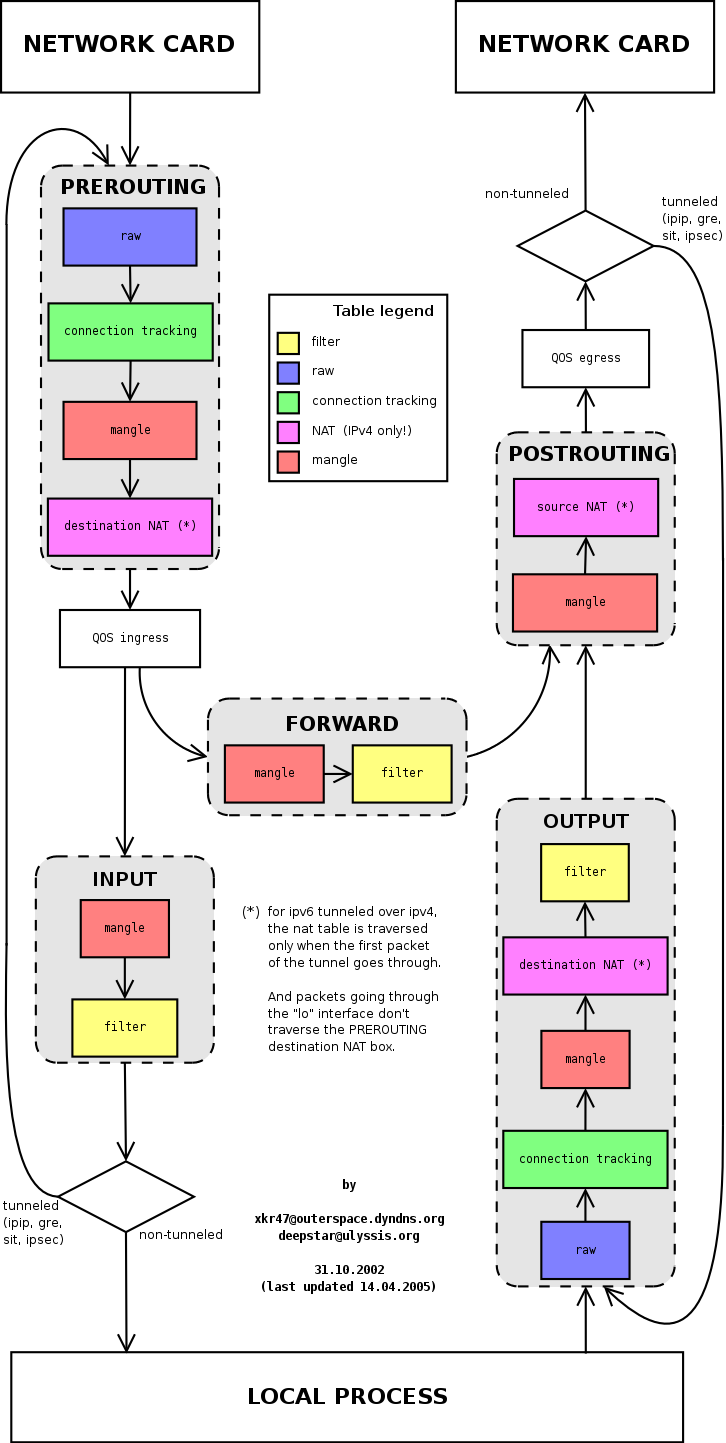
\includegraphics[width=.8\textwidth]{./pic/net.png}
\end{center}
\subsubsection{Hook函数开发}
\subsubsection{Netlink通信机制}
\subsubsection{Conntrack技术}
\subsection{HTTP协议介绍}
\subsubsection{HTTP协议基本介绍}
\subsubsection{HTTP连接管理}
HTTP definitive Guide Chap4
\begin{center}
  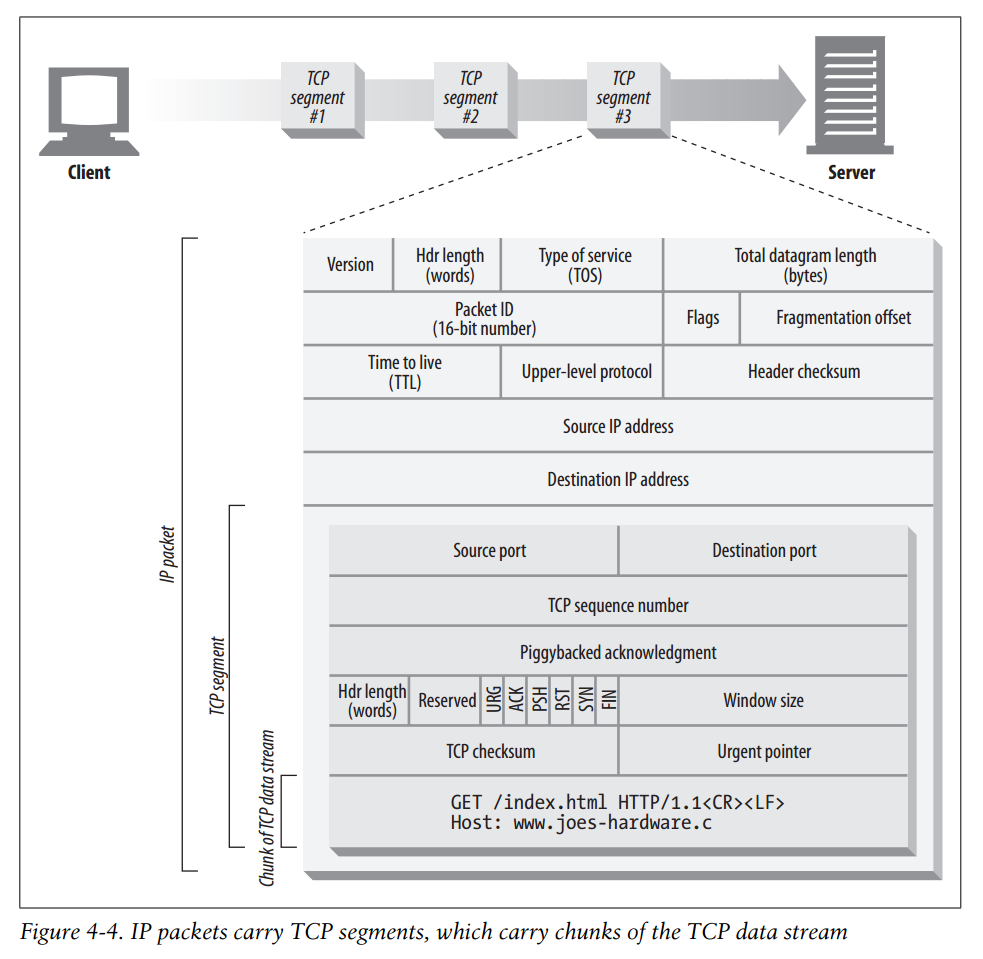
\includegraphics[width=.8\textwidth]{./pic/tcp_segment_data.png}
\end{center}
\section{OpenWRT恶意流量过滤系统的设计与实现}
\subsection{OpenWRT系统及开发介绍}
\subsection{URL请求识别系统的设计}
\subsection{Conntrack系统拓展设计}
\section{环境搭建、测试与分析}
\section{总结与展望}
\end{document} 